\documentclass[10pt]{article}
\usepackage{tikz}

\begin{document}

\[
\small\sf
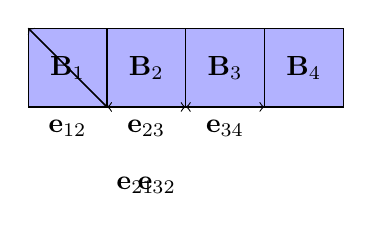
\begin{tikzpicture}[node distance=2cm]
    % Define the nodes (blue rectangles)
    \foreach \i in {1,...,4} {
        \draw[fill=blue!30] (\i,0) rectangle (\i+1,-1);
        \node at (\i+0.5,-0.5) {\(\textbf{B}_\i\)};
    }

    % Draw edges between nodes
    \draw[->] (1,0) -- (2,-1);
    \draw[->] (2,-1) -- (3,-1);
    \draw[->] (3,-1) -- (4,-1);
    \draw[->] (4,-1) -- (3,-1);
    \draw[->] (3,-1) -- (2,-1);
    \draw[->] (2,-1) -- (1,0);

    % Labeling the edges
    \node at (1.5,-1.5) [above] {\(\textbf{e}_{12}\)};
    \node at (2.5,-1.5) [above] {\(\textbf{e}_{23}\)};
    \node at (3.5,-1.5) [above] {\(\textbf{e}_{34}\)};
    \node at (3,-2) [left] {\(\textbf{e}_{32}\)};
    \node at (2,-2) [right] {\(\textbf{e}_{21}\)};
\end{tikzpicture}
\]

\end{document}